\documentclass[11pt,a4paper]{article}
%\usepackage{fontspec, xunicode, xltxtra}  
%\setmainfont{Hiragino Sans GB}  
\usepackage{xeCJK}
%\setCJKmainfont[BoldFont=STZhongsong, ItalicFont=STKaiti]{STSong}
%\setCJKsansfont[BoldFont=STHeiti]{STXihei}
%\setCJKmonofont{STFangsong}

%使用Xelatex编译

% 设置页面
%==================================================
\linespread{2} %行距
% \usepackage[top=1in,bottom=1in,left=1.25in,right=1.25in]{geometry}
% \headsep=2cm
% \textwidth=16cm \textheight=24.2cm
%==================================================

% 其它需要使用的宏包
%==================================================
\usepackage[colorlinks,linkcolor=blue,anchorcolor=red,citecolor=green,urlcolor=blue]{hyperref} 
\usepackage{tabularx}
\usepackage{authblk}         % 作者信息
\usepackage{algorithm}     % 算法排版
\usepackage{amsmath}     % 数学符号与公式
\usepackage{amsfonts}     % 数学符号与字体
\usepackage{mathrsfs}      % 花体
\usepackage{amssymb}
\usepackage[framemethod=TikZ]{mdframed}

\usepackage{graphicx} 
\usepackage{graphics}
\usepackage{color}
\usepackage{xcolor}
\usepackage{tcolorbox}
\usepackage{lipsum}
\usepackage{empheq}

\usepackage{fancyhdr}       % 设置页眉页脚
\usepackage{fancyvrb}       % 抄录环境
\usepackage{float}              % 管理浮动体
\usepackage{geometry}     % 定制页面格式
\usepackage{hyperref}       % 为PDF文档创建超链接
\usepackage{lineno}          % 生成行号
\usepackage{listings}        % 插入程序源代码
\usepackage{multicol}       % 多栏排版
%\usepackage{natbib}         % 管理文献引用
\usepackage{rotating}       % 旋转文字,图形,表格
\usepackage{subfigure}    % 排版子图形
\usepackage{titlesec}       % 改变章节标题格式
\usepackage{moresize}   % 更多字体大小
\usepackage{anysize}
\usepackage{indentfirst}  % 首段缩进
\usepackage{booktabs}   % 使用\multicolumn
\usepackage{multirow}    % 使用\multirow

\usepackage{wrapfig}
\usepackage{titlesec}     % 改变标题样式
\usepackage{enumitem}
\usepackage{aas_macros}
\usepackage{bigints}

\newcommand{\myvec}[1]%
   {\stackrel{\raisebox{-2pt}[0pt][0pt]{\small$\rightharpoonup$}}{#1}}  %矢量符号
\renewcommand{\vec}[1]{\boldsymbol{#1}}
\newcommand{\me}{\mathrm{e}}
\newcommand{\mi}{\mathrm{i}}
\newcommand{\dif}{\mathrm{d}}
\newcommand{\tabincell}[2]{\begin{tabular}{@{}#1@{}}#2\end{tabular}}

\def\kpc{{\rm kpc}}
\def\km{{\rm km}}
\def\cm{{\rm cm}}
\def\TeV{{\rm TeV}}
\def\GeV{{\rm GeV}}
\def\MeV{{\rm MeV}}
\def\GV{{\rm GV}}
\def\MV{{\rm MV}}
\def\yr{{\rm yr}}
\def\s{{\rm s}}
\def\ns{{\rm ns}}
\def\GHz{{\rm GHz}}
\def\muGs{{\rm \mu Gs}}
\def\arcsec{{\rm arcsec}}
\def\K{{\rm K}}
\def\microK{\mu{\rm K}}
\def\sr{{\rm sr}}
\newcolumntype{p}{D{,}{\pm}{-1}}

\renewcommand{\figurename}{Fig.}
\renewcommand{\tablename}{Tab.}

\renewcommand{\arraystretch}{1.5}

\setlength{\parindent}{0pt}  %取消每段开头的空格

\newcounter{theo}[section]\setcounter{theo}{0}
\renewcommand{\thetheo}{\arabic{section}.\arabic{theo}}
\newenvironment{theo}[2][]{%
\refstepcounter{theo}%
\ifstrempty{#1}%
{\mdfsetup{%
frametitle={%
\tikz[baseline=(current bounding box.east),outer sep=0pt]
\node[anchor=east,rectangle,fill=blue!20]
{\strut Theorem~\thetheo};}}
}%
{\mdfsetup{%
frametitle={%
\tikz[baseline=(current bounding box.east),outer sep=0pt]
\node[anchor=east,rectangle,fill=blue!20]
{\strut Theorem~\thetheo:~#1};}}%
}%
\mdfsetup{innertopmargin=10pt,linecolor=blue!20,%
linewidth=2pt,topline=true,%
frametitleaboveskip=\dimexpr-\ht\strutbox\relax
}
\begin{mdframed}[]\relax%
\label{#2}}{\end{mdframed}}

\newcommand*\widefbox[1]{\fbox{\hspace{2em}#1\hspace{2em}}}

\title{Hamilton力学}
\author{}
\date{\today}
\begin{document}

\maketitle

\section{Hamilton方程}
\cite{2007理论物理学教程} 利用拉格朗日函数和由它导出的拉格朗日方程来表述力学规律,先决条件是可以用广义坐标和广义速度来描述系统的力学状态。通过\textcolor{red}{勒让德变换},可以从一组\textcolor{red}{独立变量}变换到另一组。作为坐标和速度的函数的拉格朗日函数,全微分为
\begin{align*}
\dif \mathscr L &= \sum_i \frac{\partial \mathscr L}{\partial q_i} \dif q_i +\frac{\partial \mathscr L}{\partial \dot q_i} \dif \dot q_i \\
&=  \sum \dot p_i \dif q_i + \sum p_i \dif \dot q_i (\equiv \dif (\sum p_i \dif \dot q_i ) -\sum \dot q_i \dif p_i ) \\
\end{align*}
\begin{align*}
\dif (\sum p_i \dif \dot q_i -\mathscr L ) = -\sum \dot p_i \dif q_i + \sum \dot q_i \dif p_i ~.
\end{align*}
微分的变量是用广义坐标和广义动量表示系统的能量,称为系统的\textcolor{red}{Hamilton函数}:
\begin{equation}
\mathscr H (p,q,t) = \sum_i p_i \dot{q}_i - \mathscr L
\end{equation}
\begin{align}
& \dif \mathscr H = -\sum \dot p_i \dif q_i + \sum \dot q_i \dif p_i \\
\end{align}
\textcolor{red}{哈密顿方程}:
\begin{equation}
\dot q_i = \frac{\partial \mathscr H}{\partial p_i} ~, ~~\dot p_i = -\frac{\partial \mathscr H}{\partial q_i}  ~,
\end{equation}
用变量$p$和$q$表示的运动方程。它们是关于$2s$个未知函数$p_i(t)$和$q_i(t)$的$2s$个一阶微分方程组,代替拉格朗日方法的$s$个二阶方程。也称为\textcolor{red}{正则方程}。

哈密顿函数对时间的全导数为
\begin{align}
\frac{\dif \mathscr H}{\dif t} &= \frac{\partial \mathscr H}{\partial t} + \sum \frac{\partial \mathscr H}{\partial q_i} \dot q_i + \sum \frac{\partial \mathscr H}{\partial p_i} \dif \dot p_i \\
&= \frac{\partial \mathscr H}{\partial t} 
\end{align}
若哈密顿函数不显含时间,则$\dfrac{\dif \mathscr H}{\dif t} = 0$,得到能量守恒定律。

除动力学变量$q, \dot q$或$q, p$,拉格朗日函数和哈密顿函数还包含各种参数,它们与力学系统自身的性质或作用于其上的外场有关。设$\lambda$为参数,
\begin{align*}
\dif \mathscr L &= \sum \dot p_i \dif q_i +\sum p_i \dif \dot q_i + \dfrac{\partial \mathscr L}{\partial \lambda} \dif \lambda ~, \\
\dif \mathscr H &= -\sum \dot p_i \dif q_i +\sum \dot q_i \dif p_i -\dfrac{\partial \mathscr L}{\partial \lambda} \dif \lambda
\end{align*}
拉格朗日函数和哈密顿函数对参数$\lambda$的偏导数的关系
\begin{equation}
\left( \dfrac{\partial \mathscr H}{\partial \lambda} \right)_{p, q} = -\left( \dfrac{\partial \mathscr L}{\partial \lambda} \right)_{\dot q, q} ~.
\end{equation}

设拉格朗日函数的形式为$\mathscr L = \mathscr L_0 +\mathscr L^\prime$,其中$\mathscr L^\prime$是对函数$\mathscr L_0$的很小的修正。哈密顿函数$\mathscr H = \mathscr H_0 +\mathscr H^\prime$的相应附加项与$\mathscr L^\prime$的关系
\begin{equation}
\left( \mathscr H^\prime \right)_{p, q} = -\left( \mathscr L^\prime \right)_{\dot q, q} ~.
\end{equation}

拉格朗日函数和哈密顿函数对时间$t$的偏导数的关系
\begin{equation}
\left( \dfrac{\partial \mathscr H}{\partial t} \right)_{p, q} = -\left( \dfrac{\partial \mathscr L}{\partial t} \right)_{\dot q, q} ~.
\end{equation}





\section{The Hamilton Principle} 


\section{罗斯函数}









\section{泊松括号}
设$f(p, q, t)$是坐标、动量和时间的某个函数,它对时间的全导数为
\begin{align*}
\dfrac{\dif f}{\dif t} &= \dfrac{\partial f}{\partial t} + \sum_k \left(\dfrac{\partial f}{\partial q_k} \dot q_k + \dfrac{\partial f}{\partial p_k} \dot p_k \right) \\
&= \dfrac{\partial f}{\partial t} + \{H, f \} 
\end{align*}
其中
\begin{equation}
\{H, f \} = \sum_k \left(\dfrac{\partial H}{\partial p_k} \dfrac{\partial f}{\partial q_k}  -\dfrac{\partial H}{\partial q_k}  \dfrac{\partial f}{\partial p_k} \right)
\end{equation}
称为$H$和$f$的\textcolor{red}{泊松括号}。

若\textcolor{orange}{动力学变量的某个函数当系统运动时保持不变},称之为\textcolor{red}{运动积分}。$f$是运动积分的条件为
\begin{align*}
\dfrac{\dif f}{\dif t} = \dfrac{\partial f}{\partial t} + \{H, f \}  = 0
\end{align*}
若运动积分不显含时间,则
\begin{align*}
\{H, f \}  = 0
\end{align*}
\textcolor{violet}{运动积分$f$和哈密顿函数的泊松括号必等于$0$}。

对于任意一对变量$f, g$,泊松括号定义为
\begin{equation}
 \{f, g\} = \sum_k \left(\dfrac{\partial f}{\partial p_k} \dfrac{\partial g}{\partial q_k}  -\dfrac{\partial f}{\partial q_k}  \dfrac{\partial g}{\partial p_k} \right)
\end{equation}
\begin{align*}
& \{f, g\} = -\{g, f\} ~, \\
& \{f, c\} = 0 ~, \\
& \{f_1+f_2, g\} =  \{f_1, g\} + \{f_2, g\} ~, \\
& \{f_1f_2, g\} = f_1\{f_2, g\} +f_2\{f_1, g\} ~, \\
& \dfrac{\partial \{f, g\} }{\partial t} = \left\{\dfrac{\partial f}{\partial t} , g\right\} +\left\{f, \dfrac{\partial g}{\partial t}\right\} ~.
\end{align*}

若函数$f$或$g$之一是广义坐标或广义动量,则泊松括号化简为偏导数
\begin{align}
& \{f, q_k\} = \dfrac{\partial f}{\partial p_k} ~, \\
& \{f, p_k\} = -\dfrac{\partial f}{\partial q_k} ~.
\end{align}


\textcolor{red}{雅克比恒等式}:
\begin{equation}
\{f, \{g, h\} \} +\{g, \{h, f\} \} +\{h, \{f, g\} \} = 0 ~.
\end{equation}





\textcolor{red}{泊松定理}:若$f$和$g$是两个运动积分,则它们构成的泊松括号也是运动积分
\begin{equation}
 \{f, g\} = {\rm const.} 
\end{equation}
应用泊松定理,并不能总能得到新的运动积分,因为仅有$2s-1$个运动积分。在某些情况下,得到泊松括号为常数;另一些情况,新的运动积分是原来的运动积分$f$和$g$的函数。除去以上两种情况,则泊松括号给出新的运动积分。





\section{作为坐标函数的作用量}







\section{莫培督原理}





\section{正则变换}


\cite{greiner2009classical} Given a Hamiltonian $H = H(q_j, p_j, t)$, the motion of the system is found by integration of the Hamilton equations:
\begin{align}
& \dot{p}_i = -\dfrac{\partial H}{\partial q_i} ~, \\
& \dot{q}_i = \dfrac{\partial H}{\partial p_i} ~, 
\end{align}
For the case of a \textcolor{red}{cyclic coordinate}, 
\begin{align}
& \dfrac{\partial H}{\partial q_i} = 0 ~, \\
& \dot{p}_i = 0 ~, 
\end{align}
the corresponding momentum is constant: $p_i = \beta_i =$ constant. Whether or not $H$ contains cyclic coordinates depends in general on the coordinates adopted for describing a problem. A mechanical problem would be greatly simplified if one could find a coordinate transformation from the set $p_i, q_i$ to a new set of coordinates $P_i, Q_i$ with
\begin{align}
Q_i = Q_i(p_j, q_j, t) ~, \\
P_i = P_i(p_j, q_j, t) ~,
\end{align}
where all coordinates $Q_i$ for the problem were cyclic. All momenta are constant, $P_i = \beta_i$, and the new Hamiltonian $H^\prime$ is then only a function of the constant momenta $P_i$; hence, $H^\prime =H^\prime(P_j)$.
\begin{align}
& \dot{Q}_i = \dfrac{\partial H^\prime(P_j)}{\partial P_i}  = \omega_i = \rm const. ~, \\
& \dot{P}_i = -\dfrac{\partial H^\prime(P_j)}{\partial Q_i} = 0 ~,
\end{align}
\begin{align}
& Q_i =  \omega_i t + \omega_0 = \rm const. ~, \\
& P_i = \beta_i = \rm const. ~.
\end{align}
A pair $(q_i, p_i)$ is called \textcolor{red}{canonically conjugate} if the Hamilton equations hold for $q_i$ and $p_i$. The transformation from one pair of canonically conjugate coordinates to another pair is called a \textcolor{red}{canonical transformation}. In the new coordinates, Hamilton's principle is required to be maintained. For fixed instants of time, $t_1$ and $t_2$,
\begin{align}
& \delta \int_{t_1}^{t_2} L(q_j, \dot{q}_j, t) \dif t= 0 ~, \\
& \delta \int_{t_1}^{t_2} L^\prime(Q_j, \dot{Q}_j, t) \dif t = 0 ~.
\end{align}
the difference
\begin{align}
\delta \int_{t_1}^{t_2} (L-L^\prime) \dif t= 0 ~, \\
\end{align}
also vanishes. It will then be fulfilled even if the old and new Lagrangians differ by a total time derivative of a function $F$ :
\begin{equation*}
L-L^\prime = \dfrac{\dif F}{\dif t} ~,
\end{equation*}
i.e.
\begin{equation*}
\delta \int_{t_1}^{t_2} \dfrac{\dif F}{\dif t}  \dif t =  \delta(F|_{t_2} -F|_{t_1}) = 0 ~,
\end{equation*}
since the variation of a constant equals zero. The function $F$ mediates the transformation $(p_i, q_i)$ to $(P_i, Q_i)$. $F$ is  also called a \textcolor{red}{generating function}. In the general case, $F$ will be a function of the old and the new coordinates; together with the time $t$ it involves $4n + 1$ coordinates:
\begin{equation*}
F = F (p_j, q_j, P_j, Q_j, t) ~.
\end{equation*}
Since simultaneously there are $2n$ transformation equations
\begin{align}
Q_i = Q_i(p_j, q_j, t) ~, \\
P_i = P_i(p_j, q_j, t) ~,
\end{align}
$F$ involves only $2n + 1$ independent variables. $F$ must contain both a coordinate from the old coordinate set $p_i$ (or $q_i$) and one of the new $P_i$ (or $Q_i$) to enable us to establish a relation between the systems. The dependency must be selected in a suitable way, according to the actual problem.

Since 
\begin{align*}
L = \sum p_i \dot{q}_i - H = L^\prime + \dfrac{\dif F}{\dif t} = \sum P_i \dot{Q}_i - H^\prime + \dfrac{\dif F}{\dif t} ~, 
\end{align*}
For the total time derivative of $F_1$
\begin{equation*}
\dfrac{\dif F_1}{\dif t} = \sum \dfrac{\partial F_1}{\partial q_i}  \dot{q}_i + \sum \dfrac{\partial F_1}{\partial Q_i}  \dot{Q}_i + \sum \dfrac{\partial F_1}{\partial t}  ~,
\end{equation*}
\begin{equation*}
\sum p_i \dot{q}_i - \sum P_i \dot{Q}_i -H +H^\prime =  \sum \dfrac{\partial F_1}{\partial q_i}  \dot{q}_i + \sum \dfrac{\partial F_1}{\partial Q_i}  \dot{Q}_i + \sum \dfrac{\partial F_1}{\partial t} ~.
\end{equation*}
By comparing the coefficients, 
\begin{align*}
& p_i = \dfrac{\partial F_1(q_j, Q_j, t)}{\partial q_i} ~, \\
& P_i = -\dfrac{\partial F_1(q_j, Q_j, t)}{\partial Q_i} ~, \\
& H^\prime = H +\dfrac{\partial F_1(q_j, Q_j, t)}{\partial t} ~.
\end{align*}


\section{刘维尔定理}
\textcolor{red}{相空间}是以所涉及的力学系统的$s$个广义坐标和$s$个广义动量为坐标轴的$2s$维空间。相空间的每个点对应于系统的一个确定状态。当系统运动时,表示系统状态的相点在相空间中画出的曲线称为\textcolor{red}{相轨道}。
\begin{equation*}
\dif \Gamma = \dif q_1 \cdots \dif q_s \dif p_1 \cdots \dif p_s
\end{equation*}
称为相空间的``体积元"。对相空间某个区域的积分$\int \dif \Gamma$,表示这个区域的体积。这个积分值对正则变换具有不变性:\textcolor{red}{若从变量$p, q$到变量$P, Q$进行正则变换,则$p, q$空间和$P, Q$空间相应区域的体积相等},即
\begin{equation}
\color{red} \int \cdots \int \dif q_1 \cdots \dif q_s \dif p_1 \cdots \dif p_s = \int \cdots \int \dif Q_1 \cdots \dif Q_s \dif P_1 \cdots \dif P_s
\end{equation}

多重积分的变量变换为
\begin{equation*}
\int \cdots \int \dif Q_1 \cdots \dif Q_s \dif P_1 \cdots \dif P_s = \int \cdots  \int D \dif q_1 \cdots \dif q_s \dif p_1 \cdots \dif p_s
\end{equation*}
其中
\begin{equation}
\color{blue} D  = \dfrac{\partial (Q_1, \cdots, Q_s, P_1, \cdots, P_s)}{\partial (q_1, \cdots, q_s, p_1, \cdots, p_s)}
\end{equation}
称为变换的\textcolor{blue}{雅克比行列式}。即任何正则变换的雅克比行列式都等于$1$,即
\begin{equation}
\color{red} D = 1 ~.
\end{equation}

\begin{align}
\nonumber D &= \dfrac{\partial (Q_1, \cdots, Q_s, P_1, \cdots, P_s)}{\partial (q_1, \cdots, q_s, P_1, \cdots, P_s)} \Bigg/ \dfrac{\partial (q_1, \cdots, q_s, p_1, \cdots, p_s)}{\partial (q_1, \cdots, q_s, P_1, \cdots, P_s)} \\
\nonumber &= \left\{ \dfrac{\partial (Q_1, \cdots, Q_s)}{\partial (q_1, \cdots, q_s)} \right\}_{P ~= ~\rm const} \Bigg/ \left\{\dfrac{\partial (p_1, \cdots, p_s)}{\partial (P_1, \cdots, P_s)} \right\}_{q~ = ~\rm const} 
\end{align}
若``分子"和``分母"出现相同的量,则可以化为变量较少的雅克比行列式,且在计算微分时这些相同量被视为常数。分子是$s$阶行列式,其第$i$行和第$k$列的元素为$\partial Q_i/\partial q_k$,由母函数$\Phi(q, P)$进行正则变换,得到
\begin{equation}
\dfrac{\partial Q_i}{\partial q_k} = \dfrac{\partial^2 \Phi}{\partial q_k \partial P_i} ~.
\end{equation}
分母中行列式的第$i$行和第$k$列的元素为
\begin{equation}
\dfrac{\partial^2 \Phi}{ \partial q_i \partial P_k}
\end{equation}
两个行列式的差别仅仅是将行和列互换,所以二者相等。


假设在相空间中有一个小区域,其中的每个点安装力学系统的运动方程随时间运动,这个区域也整体地运动。(对于完整保守系统),这个区域的体积保持不变,即
\begin{equation}
\color{red} \dif \Gamma = \text{const.}  ~, ~~\int \dif \Gamma = \text{const.} 
\end{equation}
称为\textcolor{red}{刘维尔定理}。

积分
\begin{align*}
& J_1 = \iint \sum_i \dif q_i \dif p_k ~, \\
& J_2 = \iiiint \sum_{i \neq k} \dif q_i \dif p_i \dif q_k \dif p_k ~, \\
& \cdots ~,
\end{align*}
在正则变换下也是不变的,常称为\textcolor{yellow}{Poincare积分不变量},其积分是对相空间的给定的二维流形、四维流形进行的。

对于自由度很大的系统,通常无法准确指定系统的初始状态(即相空间中的一个确定点)。考虑系统处于相空间中各个区域的概率。令$\rho(q_0, p_0, t_0) \dif \Gamma_0$表示在$t_0$时刻系统处于$(q_0, p_0)$附近体元$\dif \Gamma_0$中的概率,$\rho(q_0, p_0, t_0)$称为概率密度。当系统按照哈密顿正则方程运动时,设在$t$时刻,$(q_0, p_0)$运动到$(q, p)$,而体积元$\dif \Gamma_0$变为包围$(q, p)$的$\dif \Gamma$。对于保守完整系统,因为相空间中不同点的相轨道不会相交,没有系统点可以进入或离开运动的体积元,因此系统处于$\dif \Gamma_0$和$\dif \Gamma$的概率是相同的,即
\begin{equation*}
\rho(q_0, p_0, t_0) \dif \Gamma_0 = \rho(q, p, t) \dif \Gamma ~.
\end{equation*}
由刘维尔定理,$\dif \Gamma_0 = \dif \Gamma$,
\begin{equation}
\rho(q_0, p_0, t_0) = \rho(q, p, t) ~,
\end{equation}
即
\begin{equation}
\dfrac{\dif \rho}{\dif t} = \dfrac{\partial \rho}{ \partial t} + [\rho, H] = 0 ~.
\end{equation}
也称为\textcolor{red}{刘维尔定理}。

考虑系统的大量的复制品,其数目应大于系统可能具有的总状态数。这些复制品具有与原系统系统相同的结构和性质,但\textcolor{red}{它们之间相互独立并具有不同的初始条件}(这些初始条件均应属于原系统的所有可能的初始条件之列)。具有上述特点的复制系统的集合称为\textcolor{red}{系综}。在特定时刻它们的状态对应于相空间中的一些点,此时\textcolor{yellow}{$\rho(q_0, p_0, t_0) \dif \Gamma_0$在差一个常数因子(系综中的总的系统数的倒数)下表示在$t_0$时刻体元$\dif \Gamma_0$中的系统数}。它等同于将系统的时间演化行为转化为用在某一时刻系综中处于某一态的系统数,进而归结为概率密度来描述。确定平衡系统的性质归结为确定概率密度$\rho(q, p, t)$。





\cite{greiner2009classical} In the Hamiltonian formalism, the \textcolor{blue}{state of motion of a mechanical system} with \textcolor{blue}{$f$ degrees of freedom at a definite time $t$} is \textcolor{blue}{completely characterized} by the specification of the \textcolor{blue}{$f$ generalized coordinates} and \textcolor{blue}{$f$ momenta $(q_1, \cdots, q_f; p_1, \cdots, p_f)$}.  These $q_i$ and $p_i$ can be understood as coordinates of a $2f$-dimensional Cartesian space, the \textcolor{red}{phase space}. The $f$-dimensional subspace of the coordinates $q_i$ is the \textcolor{red}{configuration space}; the $f$-dimensional subspace of the momenta $p_i$ is called \textcolor{red}{momentum space}. In the motion of the system the representative point describes a curve, the \textcolor{red}{phase trajectory}. If the \textcolor{red}{Hamiltonian is known}, then the \textcolor{red}{entire phase trajectory can be uniquely calculated} in advance from the coordinates of one point. \textcolor{red}{Each point belongs only one trajectory}, and \textcolor{red}{two different trajectories cannot intersect each other}. A path in phase space is given in parametric representation by $q_k(t), p_k(t) (k = 1, \cdots, f)$. Because of the \textcolor{violet}{uniqueness of the solutions of the Hamilton equations}, the \textcolor{violet}{system develops from various boundary conditions along various trajectories}. For \textcolor{orange}{conservative systems} the \textcolor{orange}{point is bound to a $(2f -1)$-dimensional hypersurface} of the phase space by the condition \textcolor{orange}{$H(q, p) = E =$ constant}.

Consider a large number $N$ of independent points that are mechanically identical, \textcolor{orange}{apart from the initial conditions}, and are described by the same Hamiltonian. If all points at time $t_1$ are distributed over a $2f$-dimensional phase space region $G_1$ with the volume
\begin{equation*}
\Delta V = \Delta q_1 \cdots \Delta q_f \cdot \Delta p_1 \cdots \Delta p_f ~,
\end{equation*}
define the density
\begin{equation*}
\rho = \dfrac{\Delta N}{\Delta V} ~.
\end{equation*}
With the course of motion, $G_1$ transforms according to the Hamilton equations into the region $G_2$. 

%===========================================================================================================================
\begin{figure}
\centering
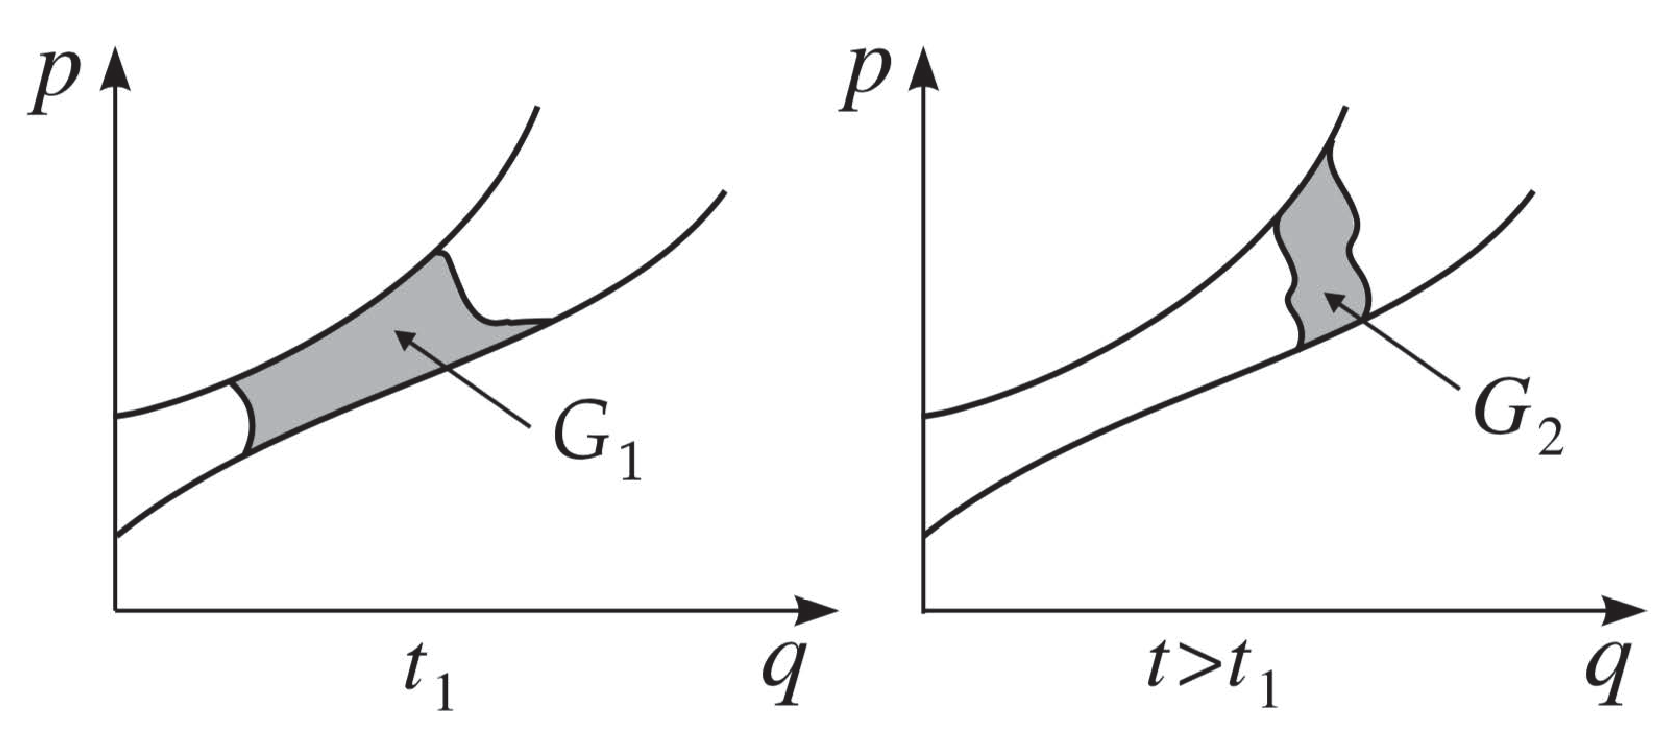
\includegraphics[height=5.cm,angle=0]{Evolution.eps}
\caption{
Evolution of a region in phase space.
} 
\label{fig:evolution}
\end{figure}
%===========================================================================================================================


\begin{tcolorbox}[colback=green!5,colframe=green!40!black,title= Liouville theorem]
The volume of an arbitrary region of phase space is conserved if the points of its boundary move according to the canonical equations.
\end{tcolorbox}
\begin{tcolorbox}[colback=green!5,colframe=green!40!black,title= Liouville theorem]
The density of points in phase space in the vicinity of a point moving with the fluid is constant.
\end{tcolorbox}
Investigate the motion of system points through a volume element of the phase space. Consider the components of the particle flux along the $q_k$- and $p_k$-direction. The area $ABCD$ represents the projection of the $2f$-dimensional volume element $\dif V$ onto the $q_k, p_k$-plane. 

%===========================================================================================================================
\begin{figure}
\centering
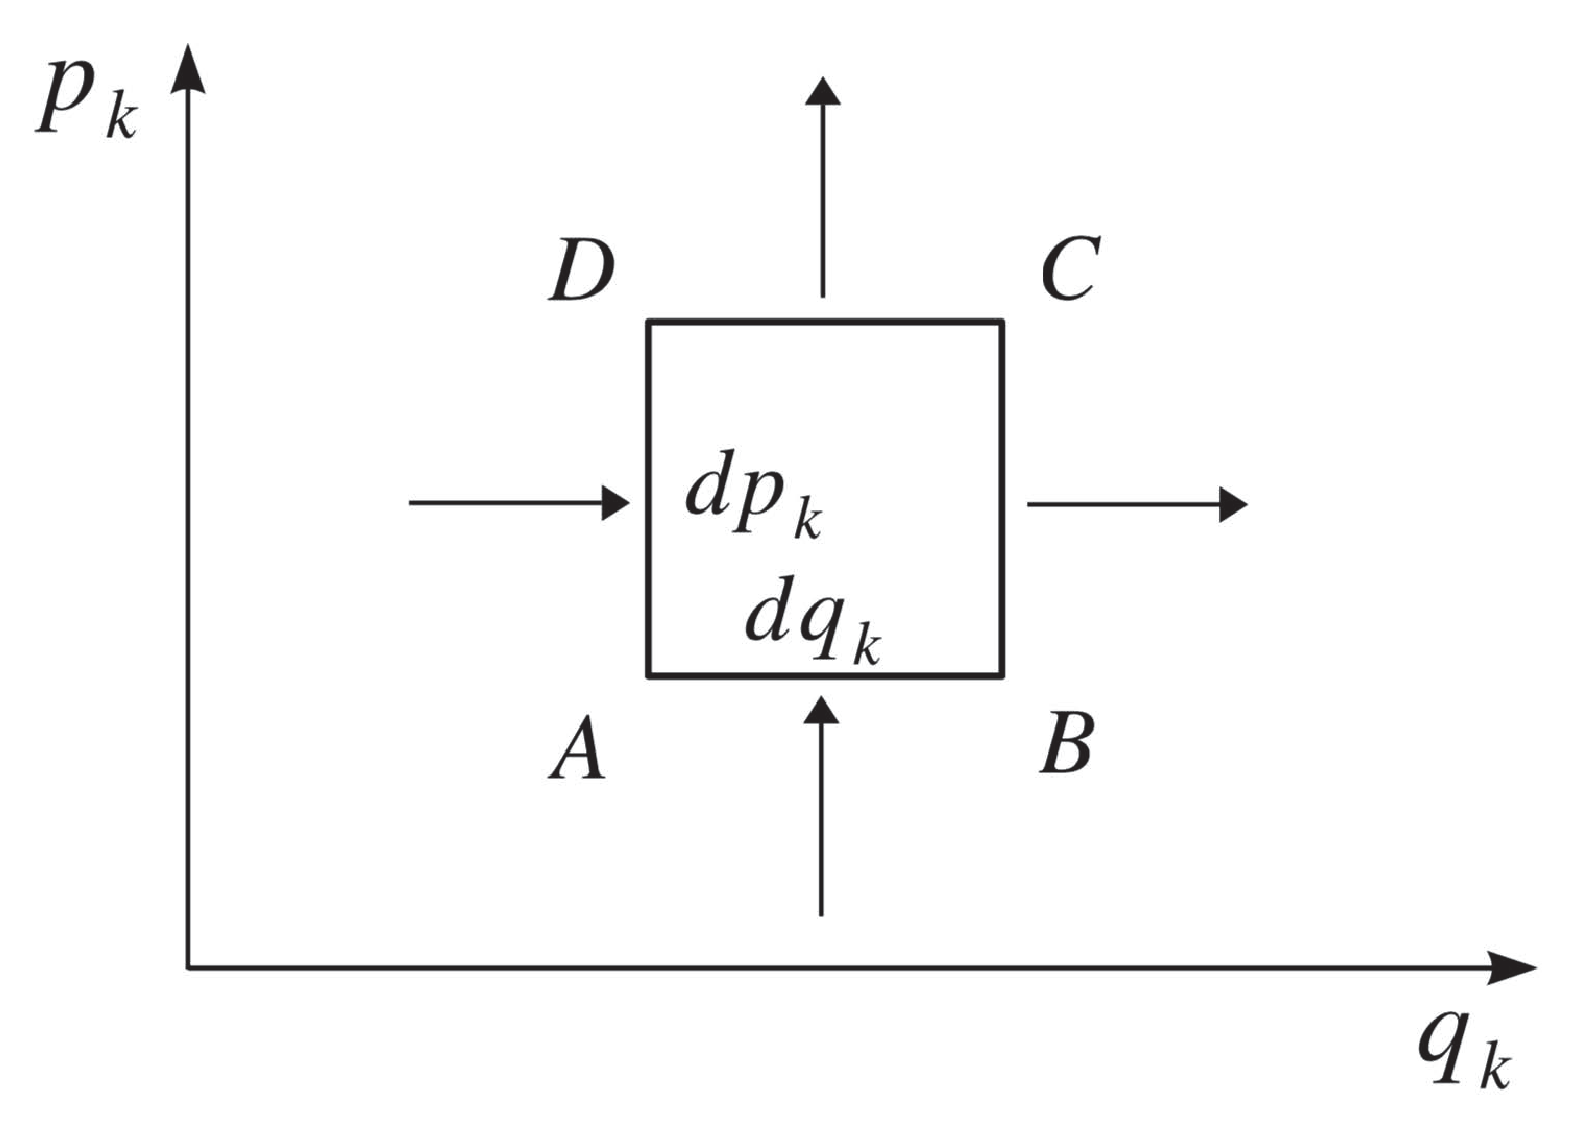
\includegraphics[height=5.cm,angle=0]{Projection.eps}
\caption{
Projection of the volume element onto the $q_k$, $p_k$-plane.
} 
\label{fig:evolution}
\end{figure}
%===========================================================================================================================

The \textcolor{orange}{number of points entering the volume element per unit time} through the ``side face" (with the projection $AD$ onto the $q_k, p_k$-plane) is
\begin{equation*}
\rho \dot{q}_k \dif p_k \cdot \dif V_k ~,
\end{equation*}
where
\begin{equation*}
\dif V_k = \prod^f_{\alpha = 1 \atop \alpha \neq k} \dif q_\alpha \dif p_\alpha 
\end{equation*}
is the $(2f - 2)$-dimensional remainder volume element. $\dif p_k \cdot \dif V_k$ is the magnitude of the lateral surface with the projection $AD$ in the $p_k, q_k$-plane. The Taylor expansion for the points leaving at $BC$ in the first direction yields
\begin{equation*}
\left( \rho \dot{q}_k + \dfrac{\partial (\rho \dot{q}_k)}{\partial q_k}  \dif q_k \right) \dif p_k \cdot \dif V_k ~.
\end{equation*}
For the flux in $p_k$-direction
\begin{align*}
& \text{entrance through} ~AB : ~~ \rho \dot{p}_k \dif q_k \cdot \dif V_k ~, \\ 
& \text{exit through} ~CD : ~~ \left( \rho \dot{p}_k + \dfrac{\partial (\rho \dot{p}_k)}{\partial p_k}  \dif p_k \right) \dif q_k \cdot \dif V_k
\end{align*}
From the flux components in $p_k$- and $q_k$-direction, the number of system points per unit time
\begin{equation}
-\left(\dfrac{\partial (\rho \dot{q}_k)}{\partial q_k} +\dfrac{\partial (\rho \dot{p}_k)}{\partial p_k} \right) \dif V
\end{equation}
gets stuck in the volume element. By summing over all $k = 1, \cdots , f$, one obtains the number of points that get stuck
in total. This quantity just corresponds to the change with time (time derivative) of the density multiplied by $\dif V$.
\begin{align}
& \dfrac{\partial \rho}{ \partial t} = -\sum_{k=1}^f \left(\dfrac{\partial (\rho \dot{q}_k)}{\partial q_k} +\dfrac{\partial (\rho \dot{p}_k)}{\partial p_k} \right) \\
& \dfrac{\partial \rho}{ \partial t} + \sum_{k=1}^f \left(\dfrac{\partial \rho}{\partial q_k} \dot{q}_k +\rho \dfrac{\partial \dot{q}_k}{\partial q_k} +\dfrac{\partial \rho}{\partial p_k}\dot{p}_k +\rho \dfrac{\partial \dot{p}_k}{\partial p_k} \right) = 0 \\
\nonumber & \dfrac{\partial \rho}{ \partial t} + \nabla \cdot (\rho \dot{\vec{r}}) = 0 
\end{align}
Where the divergence refers to the $2f$-dimensional phase space:
\begin{equation*}
\nabla = \sum_{k=1}^f \dfrac{\partial }{\partial q_k} + \sum_{k=1}^f \dfrac{\partial }{\partial p_k} ~.
\end{equation*}
From the Hamilton equations, 
\begin{align*}
& \dfrac{\partial \dot{q}_k}{\partial q_k} = \dfrac{\partial^2 H}{\partial q_k \partial p_k} ~, \\
& \dfrac{\partial \dot{p}_k}{\partial p_k} = -\dfrac{\partial^2 H}{\partial q_k \partial p_k} ~.
\end{align*}
If the second partial derivatives of $H$ are continuous, 
\begin{equation*}
\dfrac{\partial \dot{q}_k}{\partial q_k} +  \dfrac{\partial \dot{p}_k}{\partial p_k} = 0 ~,
\end{equation*}
\begin{align}
\color{red} \dfrac{\partial \rho}{ \partial t} + \sum_{k=1}^f \left(\dfrac{\partial \rho}{\partial q_k} \dot{q}_k +\dfrac{\partial \rho}{\partial p_k}\dot{p}_k \right) = 0  \Longrightarrow 
 \dfrac{\dif \rho}{\dif t} = 0 ~.
\end{align}
hence \textcolor{red}{$\rho =$ constant}.

\cite{marion1965classical, Thornton} The generalized coordinates $g_j$ can be used to define an $s$-dimensional configuration space in which every point represents a certain state of the system. Similarly, the generalized momenta $p_j$ define an $s$-dimensional momentum space in which every point represents a certain condition of motion of the system. The phase space occupied by an ensemble of particles in the absence of friction behaves like an incompressible fluid. A $2s$-dimensional space consisting of the $q_j$ and the $_j$ will allow the representation of both the positions and the momenta of all of the particles. This generalization is called \textcolor{red}{Hamiltonian phase space} or simply \textcolor{red}{phase space}. 

If, at a given instant of time, the positions and momenta of all of the particles in a system are known, then with these quantities as initial conditions the subsequent motion of the system is completely determined. That is, starting from a point $q_j(0), p_j(0)$ in phase space, the representative point which describes the system moves along a unique phase path.

For a large collection of particles, say, gas molecules, we are unable to identify the particular point in phase space that correctly represents the system. However, we may fill the phase space with a collection of points, each of which represents a possible condition of the system. We imagine a large number of systems (each consistent with the known constraints), any of which could conceivably be the actual system. Since we are unable to discuss the details of the motion of the particles in the actual system, we substitute a discussion of an ensemble of equivalent systems. Each representative point in phase space corresponds to a single system of the ensemble and the motion of a particular point represents the independent motion of that system. No two of the phase paths may ever intersect. 

Consider the representative points to be sufficiently numerous that we can define a density in phase $\rho$. The volume elements of the phase space which we use to define the density must be sufficiently large to contain a large number of representative points, but they must also be sufficiently small so that the density may be considered to vary in a continuous manner. The number $N$ of systems whose representative points lie within a volume dv of phase space is
\begin{equation}
N = \rho \dif v ~,
\end{equation}
where
\begin{equation}
\dif v = \dif q_1 \dif q_2 \cdot \dif q_s \dif p_1 \dif p_2 \cdot \dif p_s ~.
\end{equation}
$s$ is the number of degrees of freedom of each system in the ensemble.

Consider an element of area in the $q_k-p_k$ plane in phase space, as in Fig. \ref{fig:representative_points}. The number of representative points moving into $\dif q_k \dif p_k$ per unit time is
\begin{equation}
\rho (\dot{q}_k \dif p_{k} + \dot{p}_k \dif q_k) ~.
\end{equation}
By a Taylor series expansion, the number of representative points moving out of the area per unit time is (approximately)
\begin{equation}
\left(\rho \dot{q}_k + \dfrac{\partial (\rho \dot{q}_k)}{\partial q_k} \dif q_k \right) \dif p_k + \left(\rho \dot{p}_k + \dfrac{\partial (\rho \dot{p}_k)}{\partial p_k} \dif p_k \right) \dif q_k ~.
\end{equation}
The total increase in density in $\dif q_k \dif p_k$ per unit time is
\begin{align}
& \dfrac{\partial \rho}{\partial t} \dif q_k \dif p_k = - \left(\dfrac{\partial (\rho \dot{p}_k)}{\partial p_k} + \dfrac{\partial (\rho \dot{q}_k)}{\partial q_k} \right) \dif q_k\dif p_k \\
& \dfrac{\partial \rho}{\partial t} + \sum_{k=1}^s \left(\dfrac{\partial (\rho \dot{p}_k)}{\partial p_k} + \dfrac{\partial (\rho \dot{q}_k)}{\partial q_k} \right) = 0 ~.
\end{align}
Now, from Hamilton's equations, (if the second partial derivatives of $H$ are continuous)
\begin{equation}
\dfrac{\partial (\dot{p}_k)}{\partial p_k} + \dfrac{\partial (\dot{q}_k)}{\partial q_k} = 0 ~,
\end{equation}
\begin{align}
& \dfrac{\partial \rho}{\partial t} + \sum_{k=1}^s \left(\dfrac{\partial \rho}{\partial p_k} \dfrac{\dif p_k}{\dif t} + \dfrac{\partial \rho}{\partial q_k} \dfrac{\dif q_k}{\dif t} \right) = 0 ~, \\
& \dfrac{\dif \rho}{\dif t} = 0.
\end{align}
which is known as Liouville's theorem and states that the density of representative points in phase space corresponding to the motion of a system of particles remains constant during the motion.

We have been able to establish the invariance of the density $\rho$ only because the problem was formulated in phase space; an equivalent theorem for configuration space does not exist. Thus, \textcolor{yellow}{it is necessary to use Hamiltonian dynamics (rather than Lagrangian dynamics) for the discussion of ensembles in statistical mechanics.}

%===========================================================================================================================
\begin{figure}
\centering
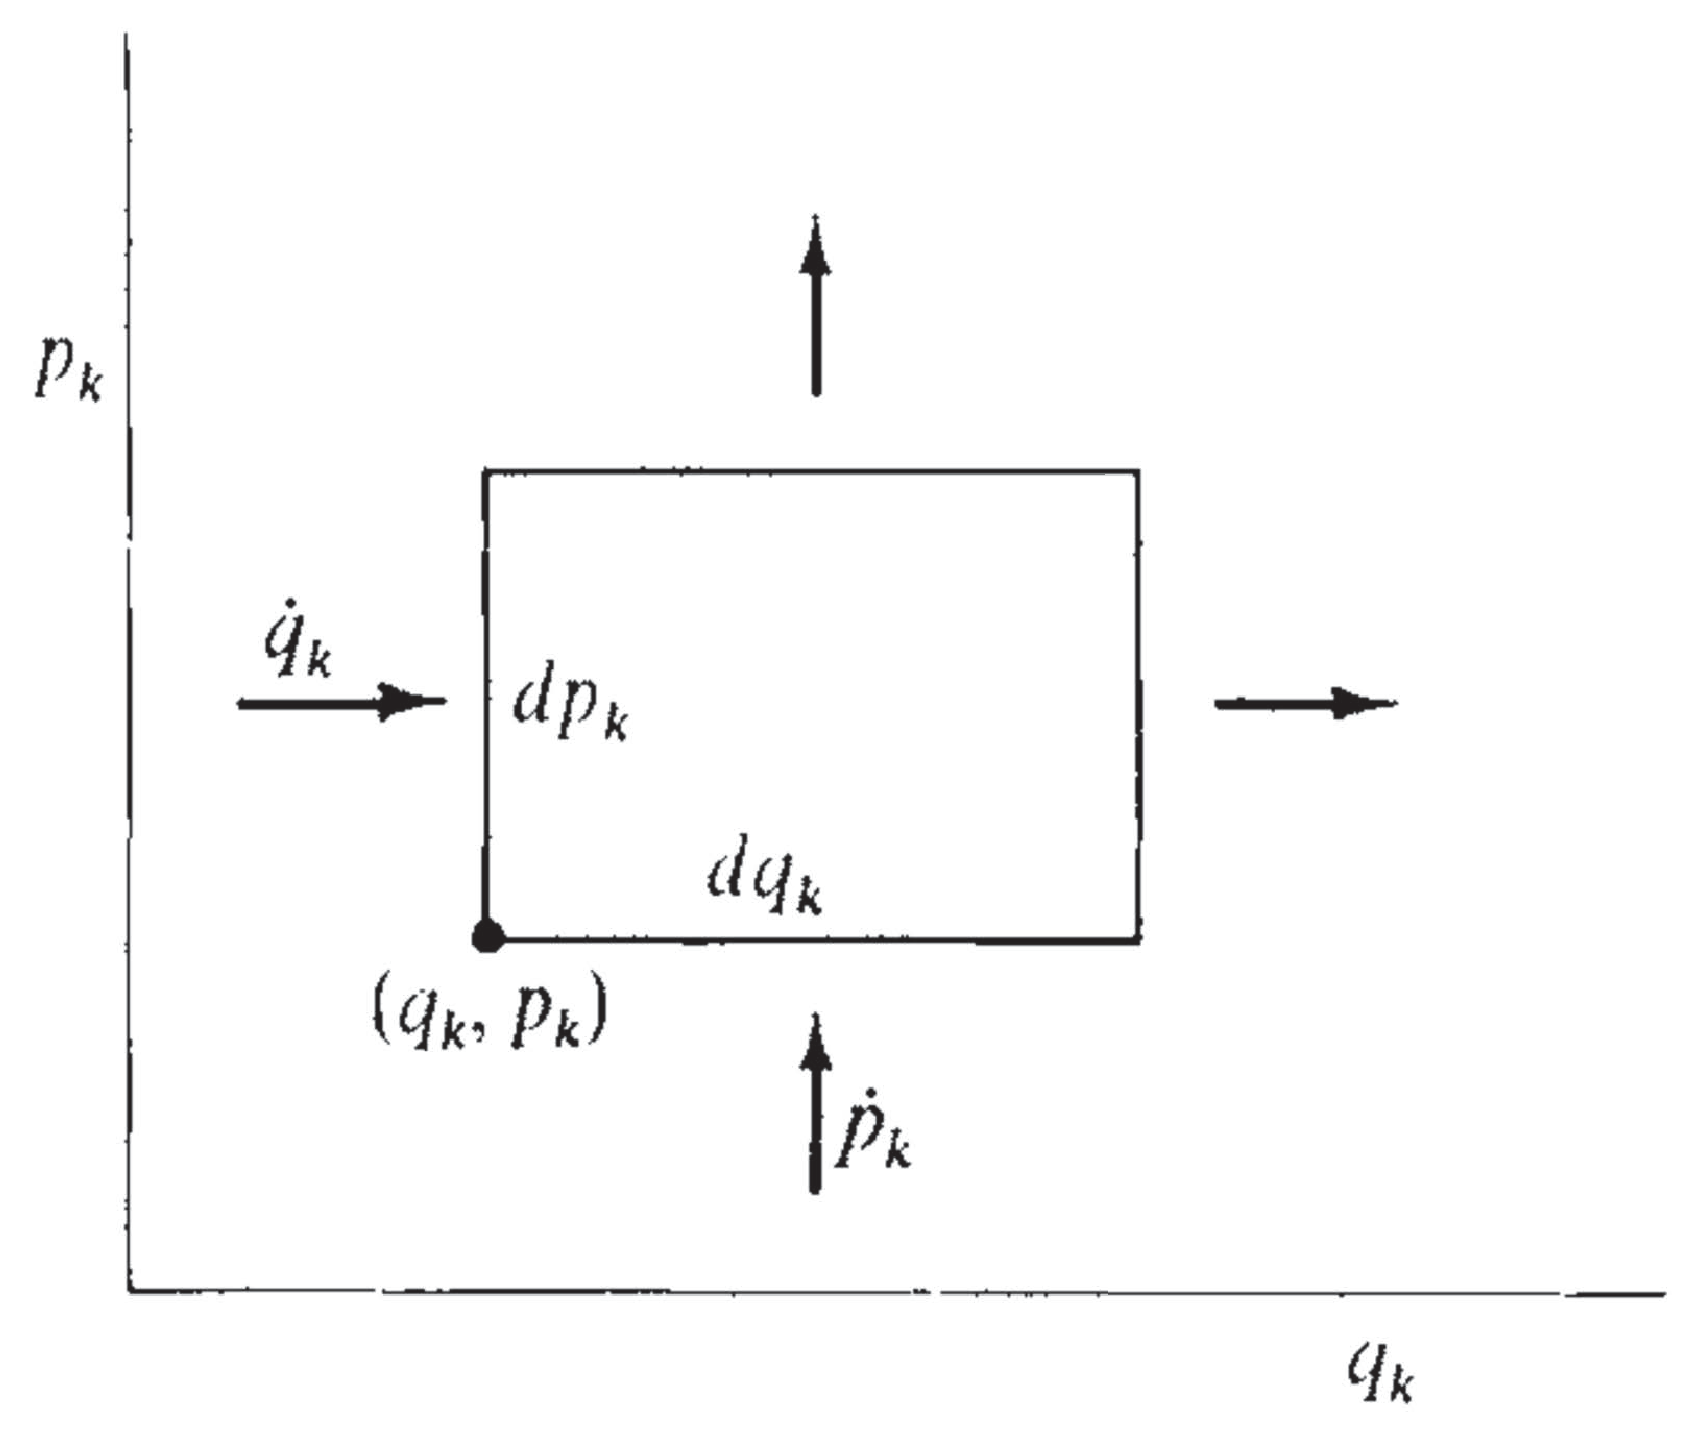
\includegraphics[height=8.cm,angle=0]{representative_points.eps}
\caption{
} 
\label{fig:representative_points}
\end{figure}
%===========================================================================================================================



\cite{2002clme.book.....G}

\section{The Principle of Stochastic Cooling}
\cite{greiner2009classical} 




\section{The Virial Theorem}
\cite{marion1965classical, Thornton} Consider a collection of particles whose position vectors $\vec{r}_a$ and whose momenta $\vec{p}_a$ are both \textcolor{red}{bounded} (i.e., \textcolor{red}{remain finite for all values of the time}). Define
\begin{equation}
\color{red} S \equiv \sum_a \vec{p}_a \cdot \vec{r}_a ~.
\end{equation}
The time derivative of $S$ is
\begin{equation}
\dfrac{\dif S}{\dif t} = \sum_a (\vec{p}_a \cdot \dot{\vec{r}}_a +\dot{\vec{p}}_a \cdot \vec{r}_a) ~.
\label{eq:dSdt}
\end{equation}
Calculate the average value of $\dif S/\dif t$ over a time interval $\tau$,
\begin{equation}
\left\langle \dfrac{\dif S}{\dif t} \right\rangle = \dfrac{1}{\tau} \int_0^\tau \dfrac{\dif S}{\dif t} \dif t = \dfrac{S(\tau) -S(0)}{\tau} ~.
\end{equation}
In the event that the motion of the system is periodic, and if $\tau$ is some integral multiple of the period, then $S(\tau) = S(0)$, and $\langle \dot{S} \rangle$ vanishes. However, even if the system does not exhibit any periodicity, since $S$ is by hypothesis a bounded function, we may make $\langle \dot{S} \rangle$ as small as desired by \textcolor{red}{allowing the time $\tau$ to become sufficiently long}. Therefore, the time average of Eq. (\ref{eq:dSdt}) can always be made to vanish (or at least to approach zero). In this limit,
\begin{equation}
\left\langle \sum_a \vec{p}_a \cdot \dot{\vec{r}}_a \right\rangle = - \left\langle \sum_a \dot{\vec{p}}_a \cdot \vec{r}_a \right\rangle
\end{equation}
On the left-hand side of this equation, $\vec{p}_a\cdot \dot{\vec{r}}_a$ is twice the kinetic energy; on the right-hand side, $\dot{\vec{p}}_a$ is just the force $\vec{F}_a$ on the $a$-th particle. 
\begin{equation}
\left\langle 2 \sum_a T_a \right\rangle = - \left\langle \sum_a \vec{F}_a \cdot \vec{r}_a \right\rangle ~.
\end{equation}
The sum over $T_a$ is the total kinetic energy $T$ of the system.
\begin{equation}
\left\langle T \right\rangle = -\dfrac{1}{2} \left\langle \sum_a \vec{F}_a \cdot \vec{r}_a \right\rangle ~.
\end{equation}
The right-hand side of this equation was called by Clausius the \textcolor{red}{virial of the system}, and the \textcolor{red}{virial theorem} is stated as: \textcolor{red}{the average kinetic energy of a system of particles is equal to its virial.}

The virial theorem is particularly useful in the kinetic theory of gases; the equation of state of a perfect gas (Boyle's law) can be derived with only a few additional considerations.

If the forces $\vec{F}_a$ can be derived from potentials $U_a$, 
\begin{equation}
\left\langle T \right\rangle = \dfrac{1}{2} \left\langle \sum_a  \vec{r}_a \cdot \textbf{grad} ~U_a \right\rangle ~.
\end{equation}
For two particles which interact according to a central, power-law force : $F \propto r^n$, the potential is
\begin{equation}
U = k r^{n+1} ~.
\end{equation}
\begin{equation}
\vec{r}_a \cdot \textbf{grad} ~U_a = r \dfrac{\dif U}{\dif r} = k (n+1) r^{n+1} = (n+1) U ~,
\end{equation}
and the virial theorem becomes
\begin{equation}
\left\langle T \right\rangle = \dfrac{n+1}{2} \left\langle U \right\rangle ~.
\end{equation}
If the particles have a gravitational interaction, then $n = -2$, and
\begin{equation}
\left\langle T \right\rangle = -\dfrac{1}{2} \left\langle U \right\rangle ~.
\end{equation}













\section{分离变量}


\section{Hamilton-Jacobi方程}

守恒律

运动方程的积分



\cite{greiner2009classical} Look for a canonical transformation to coordinates $P_i = p_{i0}$ and $Q_i = q_{i0}$ which all are constant and are given by the initial conditions. When we have found such coordinates, the transformation equations are the solutions of the system in the normal position coordinates:
\begin{align*}
q_i = q_i(q_{i0}, p_{i0}, t) ~, \\
p_i = p_i(q_{i0}, p_{i0}, t) ~, 
\end{align*}
The coordinates $(P_i, Q_i)$ obey the Hamilton equations with the Hamiltonian $H^\prime(Q_i, P_i, t)$. Since the time derivatives vanish, 
\begin{align*}
\dot{P}_i = 0 = - \dfrac{\partial H^\prime}{\partial Q_i} ~, \\
\dot{Q}_i = 0 = - \dfrac{\partial H^\prime}{\partial P_i} ~, 
\end{align*}
These conditions would certainly be fulfilled by the function $H^\prime \equiv 0$. In order to perform the coordinate transformation, we need a generating function. The new Hamiltonian shall identically vanish. Then
\begin{align}
\dfrac{\partial S}{\partial t} +H\left(q_1, \cdots, q_n; p_1 = \dfrac{\partial S}{\partial q_1}, \cdots, p_n = \dfrac{\partial S}{\partial q_n}; t \right) = 0 ~. \\
\dfrac{\partial S(q_i, P_i = \beta_i, t)}{\partial t} +H\left(q_1, \cdots, q_n; \dfrac{\partial S}{\partial q_1}, \cdots, \dfrac{\partial S}{\partial q_n}; t \right) = 0 ~.
\end{align}
This is the \textcolor{red}{Hamilton-Jacobi differential equation}. The $P_i$ denote constants that are fixed by the initial conditions $p_{i0}$. By means of this differential equation we can determine $S$. This differential equation is a nonlinear partial differential equation of first order with $n + 1$ variables $q_i, t$. It is nonlinear, since $H$ depends quadratically on the momenta that enter as derivatives of the action function with respect to the position coordinates. There appear only first derivatives with respect to the $q_i$ and the time.

To get the action function $S$, we have to integrate the differential equation $n + 1$ times (each derivative $\dfrac{\partial S}{\partial q_i}, \dfrac{\partial S}{\partial t}$ requires one integration), and we thus obtain $n + 1$ integration constants. But since $S$ appears in the differential equation only as a derivative, $S$ is determined only up to a constant $a$; i.e., $S = S^\prime + a$. This means that one of the $n + 1$ integration constants must be a constant additive to $S$.
\begin{equation*}
S = S(q_1, \cdots, q_n; \beta_1, \cdots, \beta_n; t) ~,
\end{equation*}
where the $\beta_i$ are integration constants.  The requirements are
\begin{align}
& P_i = \beta_i ~, \\
& Q_i = \dfrac{\partial S}{\partial P_i} = \dfrac{\partial S(q_1, \cdots, q_n; \beta_1, \cdots, \beta_n; t)}{\partial \beta_i} = \alpha_i ~.
\end{align}
The $\beta_i, \alpha_i$ can be determined from the initial conditions.

The original coordinates result from the transformation equations as follows: From
\begin{equation*}
\alpha_i = \dfrac{\partial S(q_j, \beta_j, t)}{\partial \beta_i} ~,
\end{equation*}
follow the position coordinates
\begin{equation*}
q_i = q_i(\alpha_j, \beta_j, t) ~.
\end{equation*}
Insertion into
\begin{equation*}
p_i = \dfrac{\partial S(q_j, P_j, t)}{\partial q_i}  = p_i(q_i, \beta_i, t)
\end{equation*}
yields
\begin{equation*}
p_i = p_i(\alpha_i, \beta_i, t)
\end{equation*}
The $q_i(\alpha_j, \beta_j, t)$ and $p_i(\alpha_j, \beta_j, t)$ are known as functions of the time and of the integration constants $\alpha_j , \beta_j$. This simply means the complete solution of the many-body problem characterized by the Hamiltonian $H(q_i, p_i, t)$.

We can separate off the time dependence in $S$. If $H$ is not an explicit function of the time, $H$ represents the total energy of the system:
\begin{equation}
-\dfrac{\partial S}{\partial t} = H = E ~.
\end{equation}
From this, it follows that $S$ can be represented as
\begin{equation}
S(q_i, P_i, t) = S_0(q_i, P_i) -Et ~.
\end{equation}
To explain the meaning of $S$, we form the total derivative of $S$ with respect to time:
\begin{equation*}
\dfrac{\dif S}{\dif t} = \sum \dfrac{\partial S}{\partial q_i} \dot{q}_i +\sum \dfrac{\partial S}{\partial P_i} \dot{P}_i +\dfrac{\partial S}{\partial t} ~.
\end{equation*}
since $\dot{P}_i = 0$, 
\begin{equation*}
\dfrac{\dif S(q_i, P_i =\beta_i, t)}{\dif t} = \sum \dfrac{\partial S}{\partial q_i} \dot{q}_i +\dfrac{\partial S}{\partial t} ~.
\end{equation*}
Because
\begin{align*}
& \dfrac{\dif S(q_j, P_j =\beta_j, t)}{\dif q_i} = p_i ~, \\
& \dfrac{\partial S}{\partial q_i} = -H ~,
\end{align*}
it further follows that
\begin{equation}
\dfrac{\dif S(q_i, P_i(p_\alpha, q_\alpha), t)}{\dif t} = \sum p_i \dot{q}_i -H(q_i, p_i, t) = L(q_i, p_i, t) ~.
\end{equation}
$H$ and $L$ are not bound by restrictions; in particular they can be time-dependent. This means that $S$ is given by the time integral over the Lagrangian:
\begin{equation}
S = \int L \dif t + \rm const.
\end{equation}
Since this integral physically represents an action (energy $\cdot$ time), the term action function for $S$ is obvious. The action function differs from the time integral over the Lagrangian by at most an additive constant. However, this last relation cannot be used for a practical calculation, since as long as the problem is not yet solved, one does not know $L$ as a function of time. Moreover, $L(q_i, p_i, t)$ depends on the original coordinates $q_i, p_i$, while the $S$-function is needed in the coordinates $q_i, P_i(q_\alpha, p_\alpha)$.










The concept of the phase integral was of fundamental importance for the transition to quantum mechanics. The first clear formulation of the quantum hypothesis consisted of the requirement that the phase integral take only discrete values; hence,
\begin{equation}
J = \oint p \dif q = nh ~, ~~ n = 1, 2, 3 \cdots
\end{equation}
where $h$ is Planck's action quantum, which has the value $h = 6.6 \times 10^{-34}$ J s. 





































\section{浸渐不变量}
研究一个由某个参数$\lambda$表征并作一维有限运动的力学系统,参数$\lambda$可以确定系统本身或者系统所处外场的性质。假设参数$\lambda$在某个外因影响下随时间缓慢(浸渐地)变化,缓慢的意思是在一个运动周期$T$时间内$\lambda$的变化很小,
\begin{equation}
T \dfrac{\dif \lambda}{\dif t} \ll \lambda ~.
\end{equation}
若$\lambda$为常数,系统是封闭且具有常能量$E$,并以确定的周期$T(E)$作严格周期运动。当$\lambda$变化时,系统不再是封闭的,能量不守恒。由于$\lambda$仅缓慢变化,能量$E$的变化率$\dot{E}$也很小。若按周期$T$平均这个变化率,所得的值$\dot{E}$确定了系统能量的平缓变化率,其正比于参数的变化率$\dot{\lambda}$。缓慢变化量$E$是$\lambda$的某个函数。$E$对$\lambda$的依赖关系可以写成$E$和$\lambda$的某种组合等于常数的形式。在含有缓变参数的系统过程中保持不变的量称为\textcolor{red}{浸渐不变量}。

设$H(q, p, \lambda)$是依赖于参数$\lambda$的系统的哈密顿函数。系统能量的变化率为
\begin{equation}
\dfrac{\dif E}{\dif t} = \dfrac{\partial H}{\partial t} = \dfrac{\partial H}{\partial \lambda} \dfrac{\dif \lambda}{\dif t} 
\end{equation}
公式右边不仅依赖于缓变量$\lambda$,而且依赖于快变量$q, p$。为了确定能量的平缓变化,须按照运动周期平均等式。考虑到$\lambda$变化缓慢($\dot \lambda$变化也缓慢),
\begin{equation}
\overline{\dfrac{\dif E}{\dif t} } = \overline{ \dfrac{\partial H}{\partial \lambda} \dfrac{\dif \lambda}{\dif t} } =  \dfrac{\dif \lambda}{\dif t} \overline{ \dfrac{\partial H}{\partial \lambda} } 
\end{equation}
在被平均的函数$\dfrac{\partial H}{\partial \lambda}$中只将$q, p$看作变量,而$\lambda$不看作变量,即,对$\lambda$保持不变时系统发生的运动取平均。
\begin{equation}
\overline{ \dfrac{\partial H}{\partial \lambda} } = \frac{1}{T} \int_0^T \dfrac{\partial H}{\partial \lambda} \dif t
\end{equation}
根据哈密顿方程$\dot q = \dfrac{\partial H}{\partial p}$,
\begin{equation}
\dif t = \frac{\dif q}{\partial H/\partial p}
\end{equation}
对时间的积分可以换为对坐标的积分,且周期$T$为
\begin{equation}
T = \int_0^T \dif t = \oint \frac{\dif q}{\partial H/\partial p}
\end{equation}
$\oint $表示对坐标在一个周期内完整变化范围内的积分。
\begin{equation}
\overline{\dfrac{\dif E}{\dif t} } = \dfrac{\dif \lambda}{\dif t} \dfrac{ \bigoint \dfrac{\partial H/\partial \lambda}{\partial H/\partial p}\dif q }{ \bigoint  \dfrac{\dif q}{\partial H/\partial p} } ~,
\end{equation}
积分沿着$\lambda$为给定常数的运动轨道进行。沿着这个轨道哈密顿函数保持常值$E$,而动量是变化的坐标$q$和两个独立常参数$E, \lambda$的确定函数。将动量当作函数$p(q; E, \lambda)$,并将方程$H(p, q; \lambda) = E$对参数$\lambda$求导,得
\begin{align*}
& \dfrac{\partial H}{\partial \lambda} + \dfrac{\partial H}{\partial p} \dfrac{\partial p}{\partial \lambda} = 0 \\
& \dfrac{\partial H/\partial \lambda }{\partial H/\partial p} = -\dfrac{\partial p}{\partial \lambda}
\end{align*}
\begin{align}
\nonumber & \overline{\dfrac{\dif E}{\dif t} } = -\dfrac{\dif \lambda}{\dif t}  \dfrac{ \bigoint \dfrac{\partial p}{\partial \lambda} \dif q }{ \bigoint \dfrac{\partial p}{\partial E} \dif p } \\
\nonumber & \oint \left(\dfrac{\partial p}{\partial E} \overline{\dfrac{\dif E}{\dif t} } +\dfrac{\partial p}{\partial \lambda} \dfrac{\dif \lambda}{\dif t} \right) \dif q = 0 \\
& \overline{\dfrac{\dif I}{\dif t} } = 0
\end{align}
$I$表示沿着$E, \lambda$给定的运动轨道积分
\begin{equation}
I = \frac{1}{2\pi} \oint p \dif q ~.
\end{equation}
当参数$\lambda$变化时,在所考虑的近似下$I$保持常数,即$I$是浸渐不变量。

$I$是系统能量(和参数$\lambda$)的函数,它对能量的偏导数确定运动周期,
\begin{align}
& 2\pi \dfrac{\partial I}{\partial E} = \oint \dfrac{\partial p}{\partial E} \dif q = T ~, \\
& \dfrac{\partial E}{\partial I} = \omega ~,
\end{align}
$\omega = 2\pi /T$是系统的振动频率。

一维自由度下,相空间为坐标$p, q$的二维空间,周期运动系统的相轨道是平面上的封闭曲线。沿着这条曲线的积分是该曲线所包围的面积,
\begin{equation}
I  = \frac{1}{2\pi} \oint p \dif q = \frac{1}{2\pi} \int \dif p \dif q
\end{equation}

\section{正则变量}
设参数$\lambda$为常数,因此所讨论的系统是封闭的。作变量$q, p$的正则变换,选取$I$作为新的``动量"。母函数为表示为$q, I$的函数的``简约作用量"$S_0$。$S_0$定义为给定能量$E$和参数$\lambda$时的积分
\begin{equation}
S_0(q, E; \lambda) = \int p(q, E; \lambda) \dif q ~.
\end{equation}
对于封闭系统,$I$只是能量的函数,$S_0$也可以表示成$S_0(q, I; \lambda)$,偏导数$\left(\dfrac{\partial S_0}{\partial q} \right)_E = p$等于$I$为常数时的偏导数$\left(\dfrac{\partial S_0}{\partial q} \right)_I$。
\begin{equation}
p = \dfrac{\partial S_0(q, I; \lambda)}{\partial q} ~,
\end{equation}
相应于正则变换的第一个公式。第二个公式确定新``新坐标",用$\omega$表示,
\begin{equation}
\omega  = \dfrac{\partial S_0(q, I; \lambda)}{\partial I} ~. 
\end{equation}
$I$和$\omega$称为\textcolor{red}{正则变量},$I$称为\textcolor{red}{作用量},$\omega$称为\textcolor{red}{角变量}。

由于母函数$S_0(q, I; \lambda)$不显含时间,新的哈密顿函数$H^\prime$是用新变量表示的老$H$。$H^\prime$是表示为作用变量的函数的能量$E(I)$。相应的正则变量的哈密顿方程为
\begin{equation}
\dot I = 0 ~, ~~ \dot \omega = \dfrac{\dif E(I)}{\dif I} 
\end{equation}
角变量是时间的线性函数:
\begin{equation}
\omega =  \dfrac{\dif E(I)}{\dif I} t +~{\rm const.} = \omega(I) t  +~{\rm const.} 
\end{equation}
振动相位。

作用量$S_0(q, I)$是坐标的多值函数。每经过一个周期,$S_0(q, I)$不回到原来的值,而是有一个增量
\begin{equation}
\Delta S_0 = 2\pi I ~.
\end{equation}
在同样的时间内,角变量的增量为
\begin{equation}
\Delta \omega = \Delta \dfrac{\partial S_0}{\partial I} = \dfrac{\partial}{\partial I}  \Delta S_0 = 2\pi ~.
\end{equation}
若用正则变量$I, \omega$表示$q, p$,或者它们的任何单值函数$F(q, p)$,则$\omega$增加$2\pi$($I$不变)时,这些函数的值保持不变。用正则变量$I, \omega $表示的任何单值函数$F(q, p)$是$\omega$的周期为$2\pi$的周期函数。


对于参数$\lambda$随时间变化的非封闭系统,运动方程也可以用正则变量$I, \omega$表示。母函数$S_0$用积分
\begin{equation}
I = \frac{1}{2\pi} \oint p \dif q
\end{equation}
给定的变量$I$表示。$S_0(q, I; \lambda(t))$是先前参数$\lambda$为常数时的母函数,但用给定函数$\lambda(t)$代替常参数$\lambda$。

\begin{equation}
H^\prime = E(I; \lambda) +\dfrac{\partial S_0}{\partial t}  = E(I; \lambda) +\Lambda \dot \lambda
\end{equation}
其中
\begin{equation}
\Lambda = \left(\dfrac{\partial S_0}{\partial \lambda} \right)_{q, I} ~,
\end{equation}
在对$\lambda$微分后,$\Lambda$用$I, \omega$表示。哈密顿方程为
\begin{align}
 \dot I &= -\dfrac{\partial H^\prime}{\partial \omega}  = -\left(\dfrac{\partial \Lambda}{\partial \omega} \right)_{I, \lambda} \dot \lambda \\
 \dot \omega &= \dfrac{\partial H^\prime}{\partial I}  = \omega(I; \lambda) +\left(\dfrac{\partial \Lambda}{\partial I} \right)_{\omega, \lambda} \dot \lambda
\end{align}
$\omega = \left(\dfrac{\partial E}{\partial I} \right)_\lambda$是振动频率。

\section{浸渐不变量守恒的准确度}
函数$S_0(q, I; \lambda)$不是$q$的单值函数,当坐标变化回到初值时,$S_0$增加$2\pi I$的整数倍。导数$\Lambda = \left(\dfrac{\partial S_0}{\partial \lambda} \right)_{q, I}$是单值函数,因求导是在$I$为常值时进行的,$S_0$的增量不出现在求导结果中。当$\Lambda$用角变量$\omega$表示时是一个周期函数。周期函数的导数$\dfrac{\partial \Lambda}{\partial \omega}$对周期的平均值为$0$。对方程取平均并将$\dot \lambda$移出平均值之外(当$\lambda$仅缓慢变化),
\begin{equation}
\overline{\dot I} = -\overline{\left(\dfrac{\partial \Lambda}{\partial \omega} \right)_I} \dot \lambda = 0 ~.
\end{equation}

设当$t \rightarrow -\infty$和$t \rightarrow +\infty$时,参数$\lambda(t)$趋向于定常极限值$\lambda_{-}$和$\lambda_{+}$,浸渐不变量($t = -\infty$)的初值$\lambda_{-}$给定,求$t = +\infty$时的增量$\Delta I = \lambda_{+} -\lambda_{-}$。


\begin{equation}
\Delta I = -\int_{-\infty}^{+\infty} \dfrac{\partial \Lambda}{\partial \omega} \dot \lambda  \dif t ~.
\end{equation}
由于$\Lambda$是$\omega$的周期函数($2\pi$),其可展开为傅里叶级数:
\begin{equation}
\Lambda = \sum_{l=-\infty}^\infty e^{il\omega} \Lambda_l 
\end{equation}
由于$ \Lambda$为实数,$ \Lambda_l  =  \Lambda^\ast_{-l} $,
\begin{equation}
\dfrac{\partial \Lambda}{\partial \omega} = \sum_{l=-\infty}^\infty il e^{il\omega} \Lambda_l = 2{\rm Re} \sum_{l=1}^\infty il e^{il\omega} \Lambda_l
\end{equation}
当$\dot \lambda$足够小,$\dot \omega$是正的(它的符号与$\omega$相同),即$\omega$是时间$t$的单调函数。
\begin{equation}
\Delta I = -\int_{-\infty}^{+\infty} \dfrac{\partial \Lambda}{\partial \omega} \dfrac{\dif \lambda}{\dif t} \dfrac{\dif t}{\dif \omega} \dif \omega
\end{equation}
将$\omega$看作复变量进行积分变换。假设被积函数对于实的$\omega$没有奇点,将积分路径从实轴移到$\omega$的上半平面。此时回路绕过被积函数的奇点``连接",形成围绕奇点的环路。设$\omega_0$是最接近实轴的奇点,即有最小(正的)虚部的奇点。在积分中这个点的邻域的贡献是主要的,且级数的每一项给出包含因子$\exp (-l {\rm Im} \omega_0)$的贡献。仅保留负指数有最小值的项$(l=1)$,
\begin{equation}
\Delta I \sim \exp (-{\rm Im} \omega_0) ~.
\end{equation}
设$t_0$是相应于奇点$\omega_0$的时刻:$\omega(t_0) = \omega_0$。$|t_0|$的量级与系统变化的特征时间$\tau$相同。
\begin{equation}
{\rm Im} \omega_0 \sim \omega \tau \sim \tau/T ~.
\end{equation}
$\tau \gg T$,因此这个指数很大。$\lambda_{+} -\lambda_{-}$随着系统参数的变化率减小而指数衰减。为了确定$T/\tau$的一阶近似下的$\omega_0$(在指数中只保留$(T/\tau)^{-1}$量级的项),略去含$\dot \lambda$的小量项,
\begin{equation}
\dfrac{\dif \omega}{\dif t} = \omega(I, \lambda(t) ) ~,
\end{equation}
且将$\omega(I, \lambda(t) )$的自变量$I$取为一常数值,如$I_{-}$。
\begin{equation}
\omega_0 = \int^{t_0} \omega(I, \lambda(t) ) \dif t
\end{equation}
(积分下限可以取任意实数值$t$,因为对所要求的$\omega_0$的虚部没有影响)。
\begin{equation}
\Delta I \sim {\rm Re} \int i e^{i\omega} \frac{\dot \lambda \dif \omega}{\omega(I, \lambda) } ~.
\end{equation}
关于最接近实轴而需要考虑的奇点是函数$\dot \lambda$和$1/ \omega(t)$的奇点(极点、支点)。










































%%%%%%%%%%%%%%%%%%%%%%%%%%%%%%%%%%%%%%%%%%%%%%%%%%%%%%%%%%%%%%%%%%%%%%
\bibliographystyle{unsrt_update}
\bibliography{ref}
%%%%%%%%%%%%%%%%%%%%%%%%%%%%%%%%%%%%%%%%%%%%%%%%%%%%%%%%%%%%%%%%%%%%%%


\end{document}